% !TeX program = xelatex
\documentclass{article}
\usepackage{kotex}
\usepackage[a4paper,left=3cm, right=3cm, top=2cm, bottom=2cm]{geometry}
\usepackage{amsmath}
\usepackage{graphicx}
\usepackage{caption}
\usepackage{setspace}
\usepackage{xcolor}
\usepackage{titlesec}
\usepackage{amssymb}
\usepackage{tcolorbox}
\usepackage{wrapfig}
\usepackage{amsthm}
\usepackage{multirow} 
\usepackage{array}
\usepackage{tcolorbox}
\usepackage{pgfplots}
\pgfplotsset{compat=1.18} % For proofs

\graphicspath{{graph/}}
\title{7.3 이차곡면의 중심}
\date{}
\author{}
\setstretch{1.3}

% \subsection* 형식 지정 (번호 없음)
\titleformat{name=\section, numberless}
  {\normalfont\large\bfseries\color{blue}}
  {}
  {0pt}
  {}
\geometry{a4paper, margin=1in}

% 증명 환경 스타일
\newtheoremstyle{mystyle}% name
  {}% Space above
  {}% Space below
  {\itshape}% Body font
  {}% Indent amount
  {\bfseries}% Theorem head font
  {.}% Punctuation after theorem head
  {.5em}% Space after theorem head
  {}% Theorem head spec (can be left empty, meaning `normal')
\theoremstyle{mystyle}

\begin{document}
\maketitle

\begin{tcolorbox}[colback=blue!5, colframe=blue!60!black, title=7.3 이차곡면의 중심 -- 한눈에 보기, boxrule=0.5mm, arc=3mm]
\begin{center}
\renewcommand{\arraystretch}{1.3}
\begin{tabular}{|p{2.5cm}|p{5.5cm}|p{5.5cm}|}
\hline
\textbf{판별식 \(D\)} & \textbf{의미} & \textbf{해당 곡면} \\
\hline
\(D\ne0\) & 중심이 하나(유심이차곡면) & 타원면, 쌍곡면, 추면 \\
\hline
\(D=0\) & 중심이 무수히 많거나 없음(무심이차곡면) & 포물면, 주면류, 두 평면 \\
\hline
\end{tabular}
\end{center}
여기서 \(D=\begin{vmatrix} a&h&g\\ h&b&f\\ g&f&c \end{vmatrix}\)이다.
\end{tcolorbox}

\begin{tcolorbox}[
    colback=teal!4,
    colframe=teal!65!black,
    title=정의 \& 핵심 규칙,
    fonttitle=\bfseries,
    boxrule=0.5mm,
    arc=3mm
    ]
    \textbf{\textcolor{teal!65!black}{정의.}}\quad
    이차곡면
    \[
    F(x,y,z)=ax^2+by^2+cz^2+2fyz+2gzx+2hxy+2lx+2my+2nz+d=0
    \]
    위의 한 점을 지나는 모든 현이 항상 점 \((x_0,y_0,z_0)\)에서 이등분될 때, 이 점을 이차곡면의 \textbf{중심}이라 하고, 중심을 지나는 현을 \textbf{직경}이라 한다.

    \noindent\textcolor{teal!50!black}{\rule{\linewidth}{0.4pt}}

    \textbf{\textcolor{teal!65!black}{핵심 규칙.}}\quad
    중심을 구하는 연립방정식은
    \[
    ax_0+hy_0+gz_0+l=0,\quad hx_0+by_0+fz_0+m=0,\quad gx_0+fy_0+cz_0+n=0
    \]
    이고, 계수행렬식 \(D=\begin{vmatrix} a&h&g\\ h&b&f\\ g&f&c \end{vmatrix}\)이
    \begin{itemize}
        \item \(D\ne0\)이면 해가 유일 $\to$ \textbf{유심이차곡면} (중심 하나)
        \item \(D=0\)이면 해가 무수히 많거나 없음 $\to$ \textbf{무심이차곡면}
    \end{itemize}
\end{tcolorbox}

% ============ 이미지 삽입 위치 1: 중심과 직경 개념도 ============
% 타원면 위에 중심 O를 지나는 현(직경) P1P2를 표시.
% "중심 = 모든 현의 중점"이라는 정의를 시각적으로 보여줌.
\begin{figure}[h]
\centering
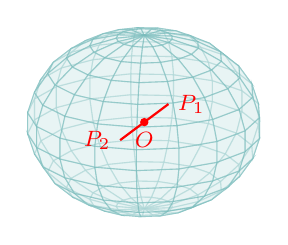
\begin{tikzpicture}
\begin{axis}[hide axis, view={115}{20}, width=5.5cm, height=5.5cm]
\addplot3[
    surf, shader=faceted, faceted color=teal!55, fill=teal!12, opacity=0.5,
    domain=0:180, domain y=0:360, samples=14, samples y=18, z buffer=sort,
]
({2*sin(x)*cos(y)}, {1.2*sin(x)*sin(y)}, {1.5*cos(x)});
\addplot3[thick, red] coordinates {(-1.7,-0.75,-1.0) (1.7,0.75,1.0)};
\addplot3[only marks, mark=*, mark size=1.3pt, red] coordinates {(0,0,0)};
\node at (axis cs:0,0,0)[anchor=north, red]{\footnotesize $O$};
\node at (axis cs:1.7,0.75,1.0)[anchor=west, red]{\footnotesize $P_1$};
\node at (axis cs:-1.7,-0.75,-1.0)[anchor=east, red]{\footnotesize $P_2$};
\end{axis}
\end{tikzpicture}
\caption{중심 $O$를 지나는 현(직경) $P_1P_2$ -- $O$는 모든 현의 중점}
\end{figure}

유도 과정을 정리하면 다음과 같다. 점 \((x_0,y_0,z_0)\)를 지나고 방향코사인이 \(\lambda,\mu,\nu\)인 직선
\[
x=x_0+\lambda t,\quad y=y_0+\mu t,\quad z=z_0+\nu t
\]
과 곡면 \(F(x,y,z)=0\)의 교점은 \\
$(a\lambda^2+b\mu^2+c\nu^2+2f\mu\nu+2g\nu\lambda+2h\lambda\mu)t^2 \\
+2\{(ax_0+hy_0+gz_0+l)\lambda+(hx_0+by_0+fz_0+m)\mu+(gx_0+fy_0+cz_0+n)\nu\}t \\
+F(x_0,y_0,z_0)=0$ \\
을 만족하는 \(t\)의 값에 따라 결정된다. 두 교점을 잇는 현의 중점이 \((x_0,y_0,z_0)\)가 되려면 이 이차방정식이 절댓값이 같고 부호가 반대인 두 근을 가져야 하므로, \(t\)의 일차항 계수가 0이어야 한다:
\[
(ax_0+hy_0+gz_0+l)\lambda+(hx_0+by_0+fz_0+m)\mu+(gx_0+fy_0+cz_0+n)\nu=0
\]
이 조건이 \textbf{모든} \(\lambda,\mu,\nu\)에 대해 성립해야 \((x_0,y_0,z_0)\)가 중심이 되므로, 앞의 연립방정식을 얻는다.

\subsection*{EXAMPLE 1}
이차곡면 \(ax^2+by^2+cz^2+d=0\)의 중심을 조사하여라.\\
\textbf{SOLUTION:} 중심을 정하는 식은 \(ax=0,\ by=0,\ cz=0\)이다. 따라서 \(a,b,c\)가 모두 0이 아니면 중심은 단 하나, 원점이다. 즉 \textbf{타원면, 쌍곡면}은 중심을 하나 가지는 이차곡면이다. 특히 이 중심이 곡면 위에 있으려면 \(d=0\)이어야 하는데, 이때의 곡면은 \textbf{추면}이다. 즉 추면은 하나의 중심을 가지되 그 중심이 곡면 위에 있다.

만일 \(a,b,c\) 중 하나나 둘이 0이면 중심은 무수히 많이 존재하며 한 직선 위 또는 한 평면 위에 있다. 즉 \textbf{타원주면, 쌍곡주면, 두 평면}은 무수히 많은 중심을 갖는 이차곡면이다.

\subsection*{EXAMPLE 2}
이차곡면 \(ax^2+by^2+2nz=0\ (n\ne0)\)의 중심을 조사하여라.\\
\textbf{SOLUTION:} 중심을 정하는 방정식은 \(ax=0,\ by=0,\ n=0\)이다. 그런데 \(n\ne0\)이므로 이 방정식을 만족하는 해가 없다. 즉 \textbf{포물면과 포물주면은 중심을 갖지 않는다.}

% ============ 이미지 삽입 위치 2: 유심 vs 무심 비교 ============
% 왼쪽: 타원면 (중심 O 존재, 유심이차곡면)
% 오른쪽: 타원포물면 (서로 다른 두 현의 중점이 일치하지 않음 → 무심이차곡면)
\begin{figure}[h]
\centering
\begin{tikzpicture}
\begin{axis}[hide axis, view={115}{20}, width=5cm, height=5cm]
\addplot3[
    surf, shader=faceted, faceted color=teal!55, fill=teal!12, opacity=0.5,
    domain=0:180, domain y=0:360, samples=14, samples y=18, z buffer=sort,
]
({1.6*sin(x)*cos(y)}, {1.1*sin(x)*sin(y)}, {1.3*cos(x)});
\addplot3[only marks, mark=*, mark size=1.3pt, red] coordinates {(0,0,0)};
\node at (axis cs:0,0,0)[anchor=north west, red]{\footnotesize $O$ (중심)};
\end{axis}
\end{tikzpicture}
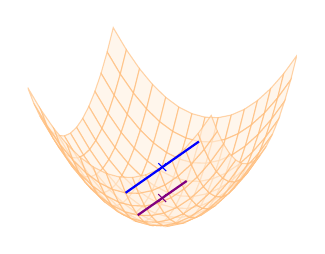
\begin{tikzpicture}
\begin{axis}[hide axis, view={115}{20}, width=5cm, height=5cm]
\addplot3[
    surf, shader=faceted, faceted color=orange!55, fill=orange!12, opacity=0.6,
    domain=-1.4:1.4, domain y=-1.4:1.4, samples=15, samples y=15,
]
{x^2+y^2};
\addplot3[thick, blue] coordinates {(-1.2,0,1.44) (1.2,0,1.44)};
\addplot3[thick, violet] coordinates {(-0.8,0,0.64) (0.8,0,0.64)};
\addplot3[only marks, mark=x, mark size=2pt, blue] coordinates {(0,0,1.44)};
\addplot3[only marks, mark=x, mark size=2pt, violet] coordinates {(0,0,0.64)};
\end{axis}
\end{tikzpicture}
\caption{왼쪽: 타원면(유심, 중심 $O$ 하나) / 오른쪽: 타원포물면(무심, 서로 다른 현의 중점 \(\times\)가 일치하지 않음)}
\end{figure}

\section*{연습문제 7.3}
\begin{enumerate}
    \item 다음 이차곡면의 중심을 구하여라.
    \begin{enumerate}
        \item[(1)] \(2x^2+4y^2-z^2-8x+8y+4=0\)
        \item[(2)] \(2x^2+y^2-z^2+4yz-2zx-4xy+2y-4z=0\)
        \item[(3)] \(3x^2+2y^2+z^2+2yz+2zx+2xy+2x-2y-2z-2=0\)
    \end{enumerate}
\end{enumerate}
\end{document}